\begin{frame}{A miniHPC}
	\begin{columns}[T]
		\begin{column}[c]{.6\textwidth}
			\begin{itemize}
				\item CarpentriesOffline started about four years go (2022 SSI Fellowship).
				\item We decided we need an HPC version too due to the difficulties associated with getting access to HPCs for training.
				\item Raspberry Pi 4s, one login node, five compute nodes, one access point
				\item The same open source software stack as many HPCs: Slurm, lmod, munge
				\item EESSI for software
				
			\end{itemize}
		\end{column}
		
		\begin{column}[c]{.5\textwidth}
			\begin{figure}
				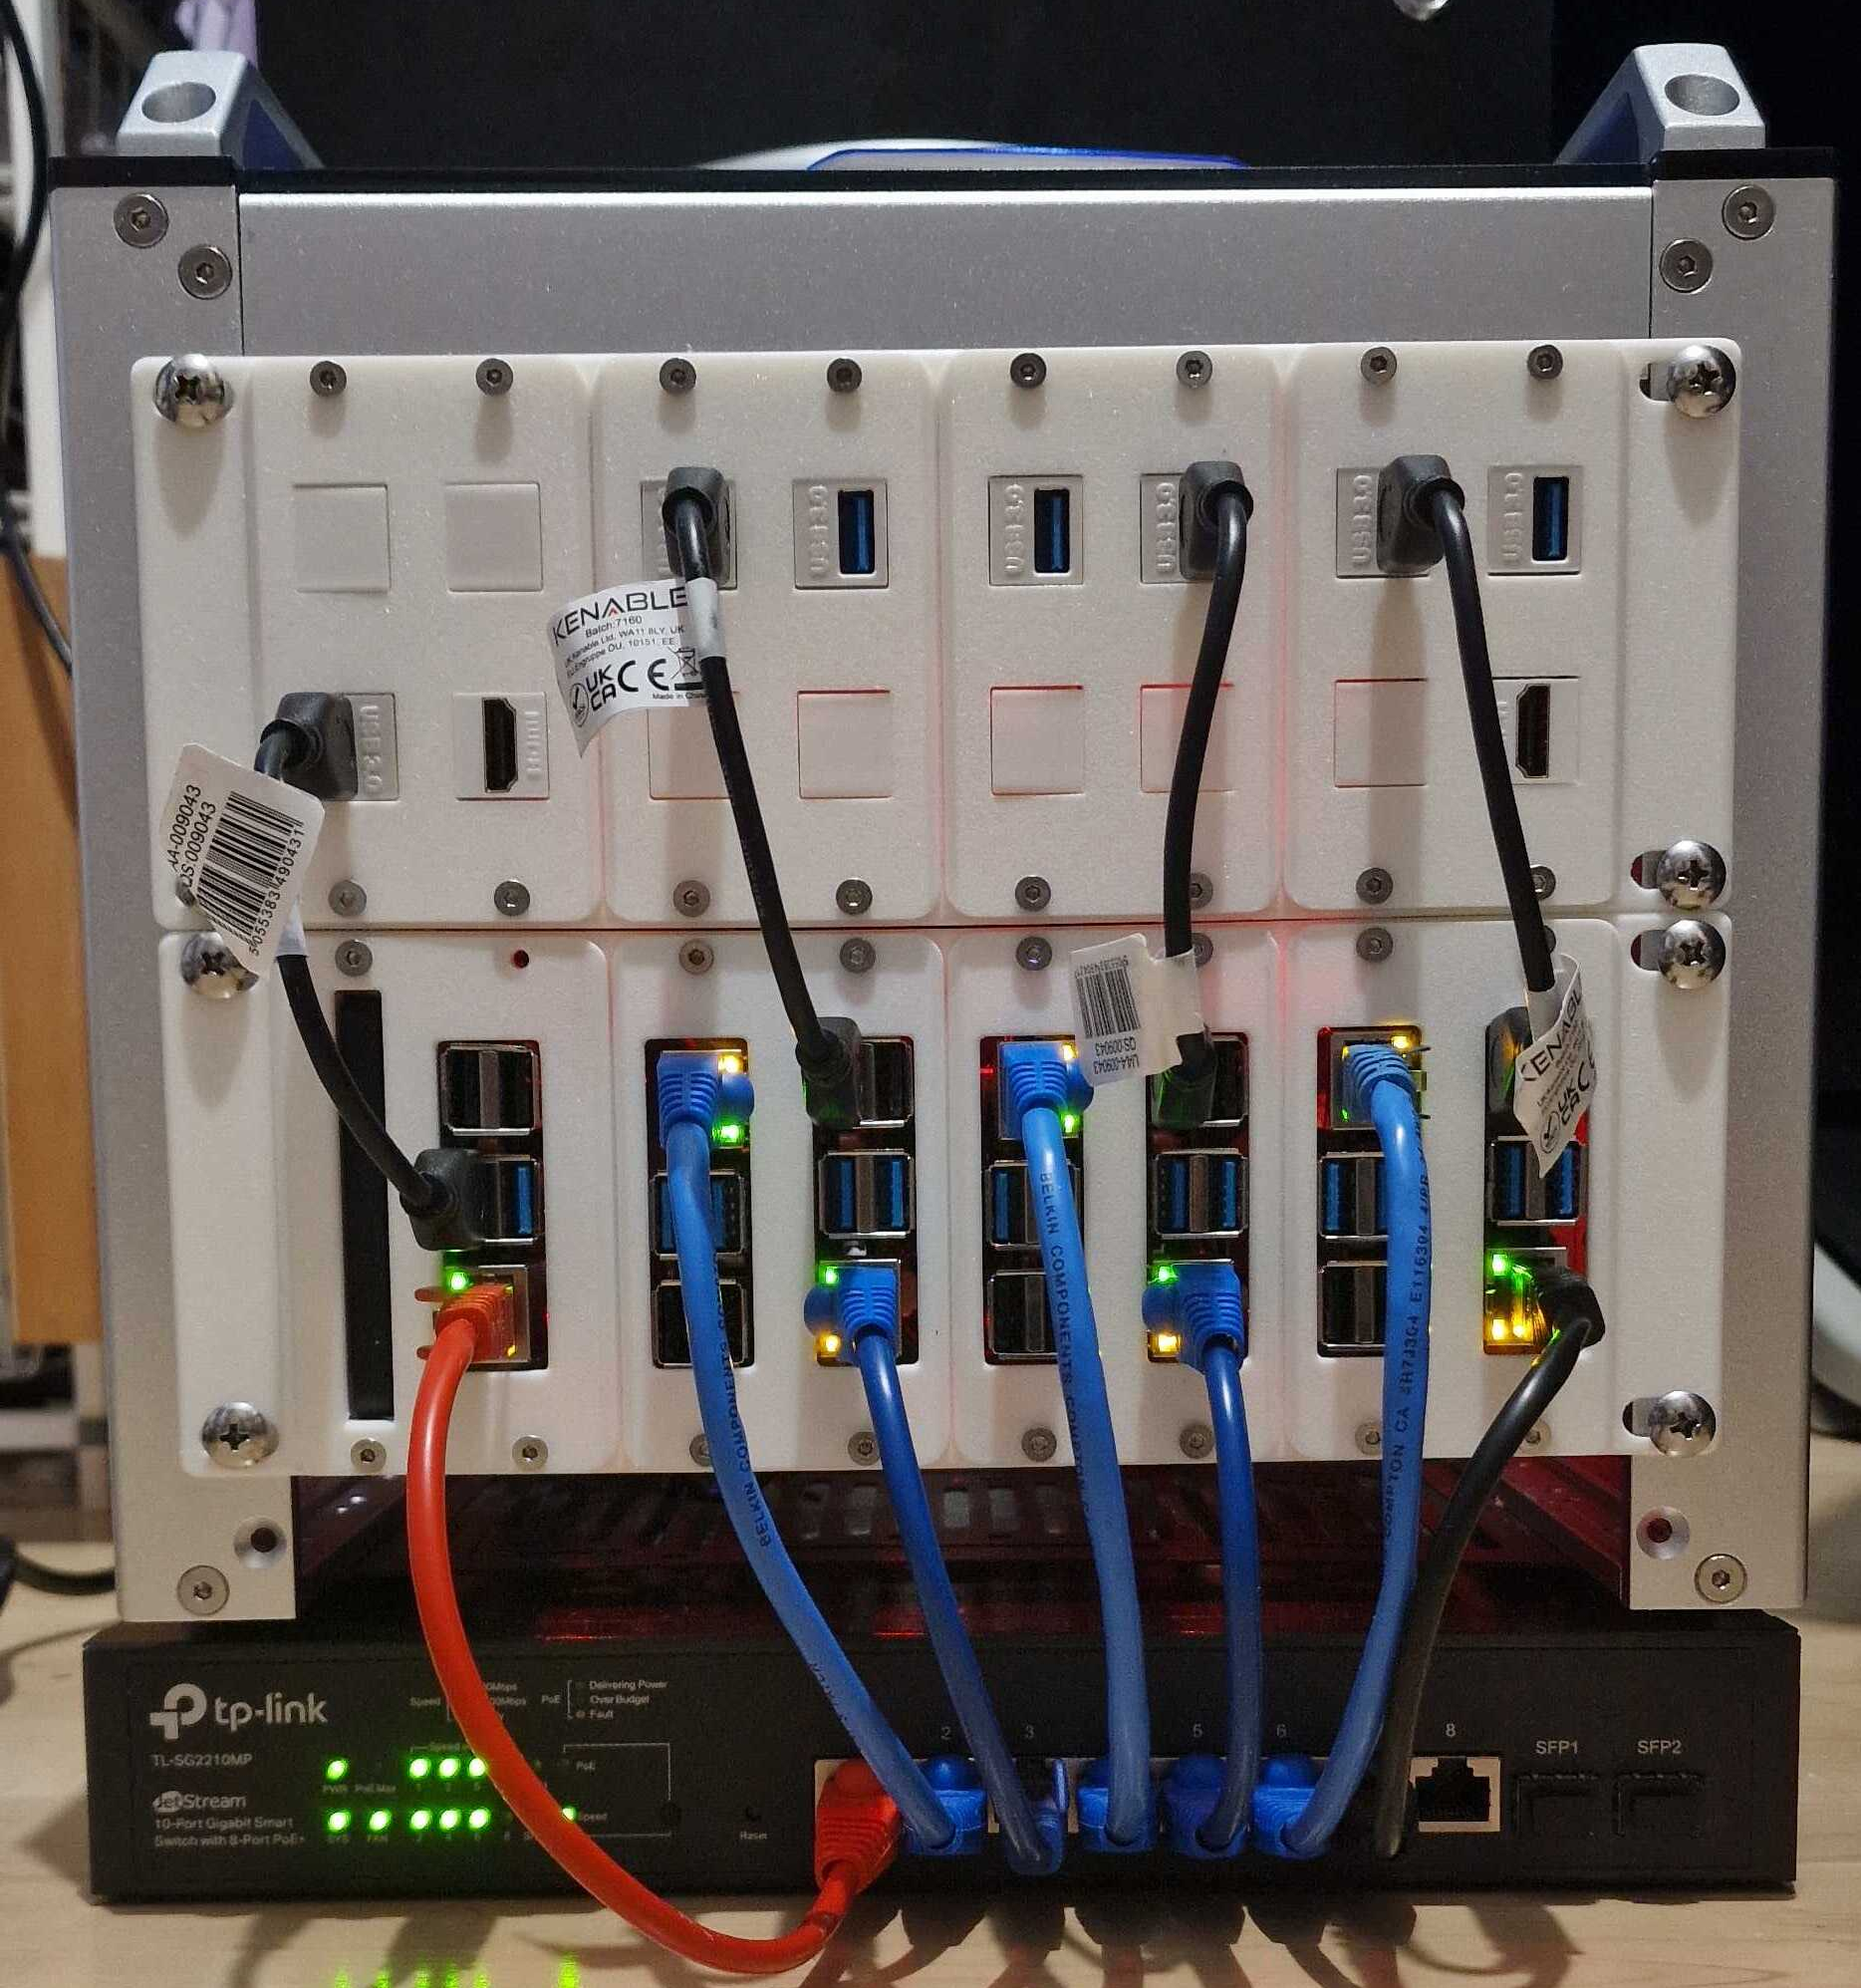
\includegraphics[width=.4\columnwidth]{images/mini-HPC-proto3.png} 
				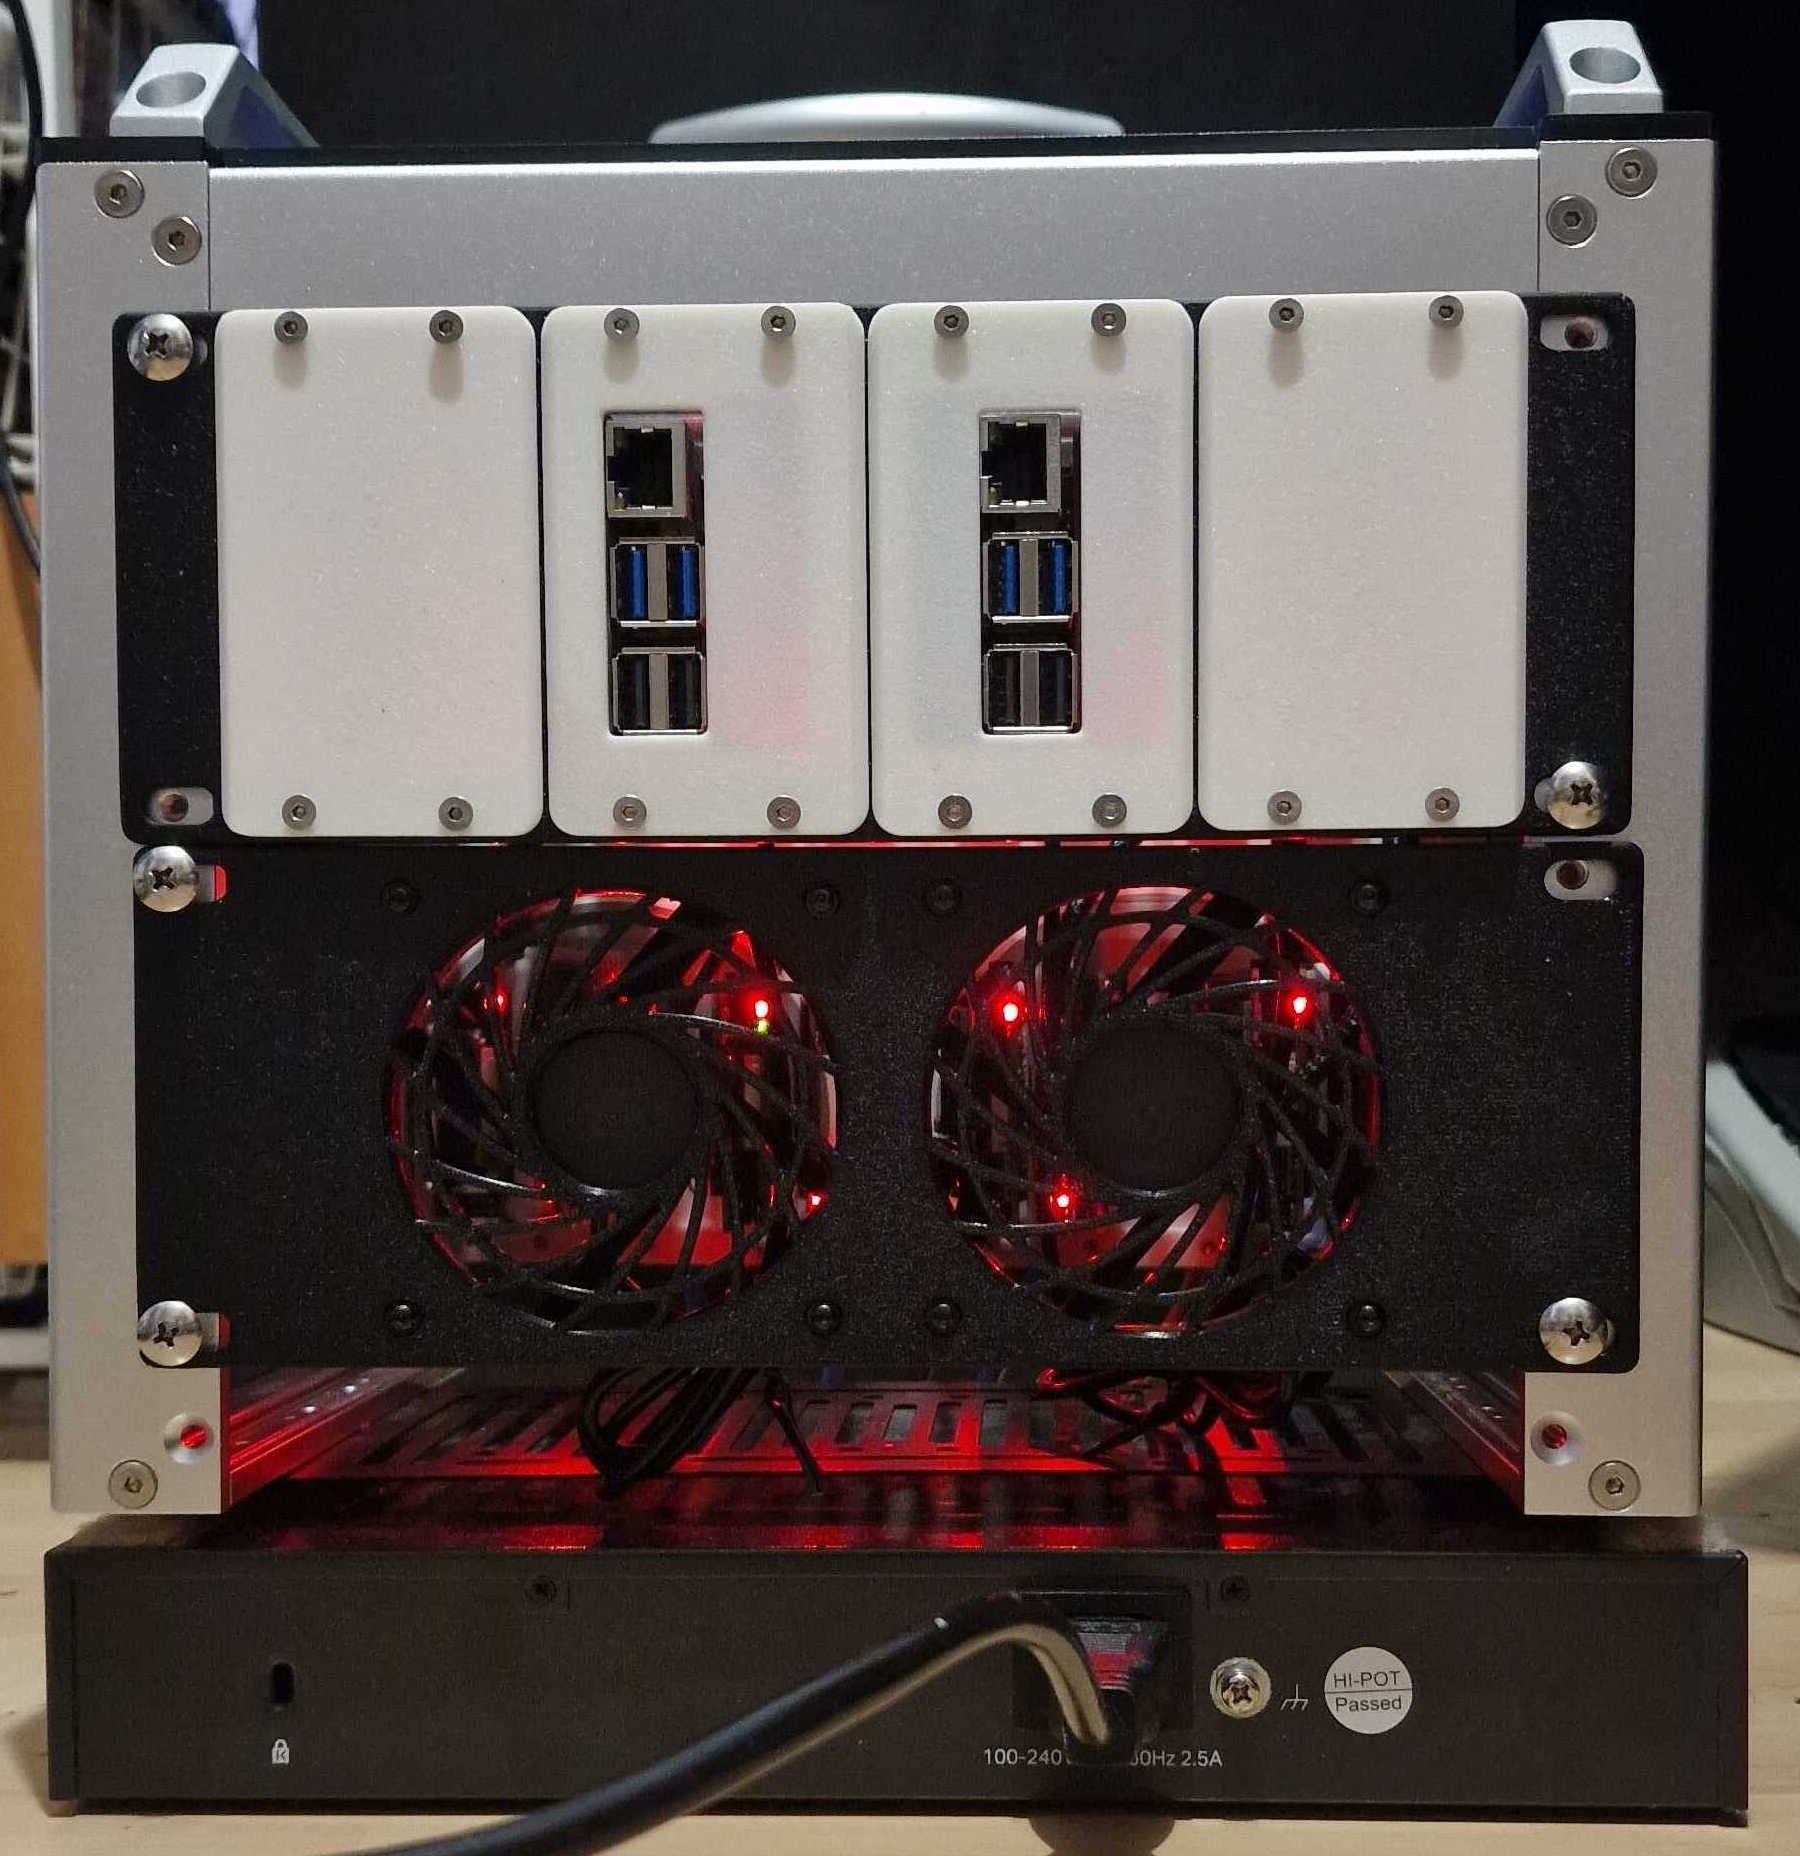
\includegraphics[width=.4\columnwidth]{images/mini-HPC-proto3_back.png}
				\caption*{Front and Back}
			\end{figure}
		\end{column}
	\end{columns}
	
\end{frame}